%% ECAI 2026 Submission
%% Compile: pdflatex paper.tex && bibtex paper && pdflatex paper.tex && pdflatex paper.tex

\documentclass[twocolumn,10pt]{article}
\usepackage[T1]{fontenc}
\usepackage[utf8]{inputenc}
\usepackage{lmodern}
\usepackage[margin=1.75cm,top=2.0cm,bottom=2.2cm,columnsep=0.55cm]{geometry}
\usepackage{graphicx}
\usepackage{amsmath,amssymb,amsthm}
\usepackage{booktabs,multirow,array,tabularx,colortbl}
\usepackage{url,xcolor}
\usepackage{paralist}
\usepackage{titlesec}
\usepackage{abstract}
\usepackage{fancyhdr}
\usepackage[numbers,sort&compress]{natbib}
\usepackage[colorlinks=true,linkcolor=NavyBlue,citecolor=NavyBlue,urlcolor=NavyBlue]{hyperref}
\usepackage{pifont}
\usepackage{microtype}

% ── TikZ (kept for any inline diagrams) ──────────────────────────────────────
\usepackage{tikz}

% ── Algorithm ───────────────────────────────────────────────────────────────
\usepackage{algorithm}
\usepackage{algorithmic}
\renewcommand{\algorithmiccomment}[1]{\hfill{\small\textit{// #1}}}

% ── Colors ──────────────────────────────────────────────────────────────────
\definecolor{NavyBlue}{RGB}{0,70,127}
\definecolor{RoyalBlue}{RGB}{65,105,225}
\definecolor{SteelBlue}{RGB}{70,130,180}
\definecolor{LightBlue}{RGB}{219,234,254}
\definecolor{DarkGreen}{RGB}{22,101,52}
\definecolor{LightGreen}{RGB}{220,252,231}
\definecolor{Amber}{RGB}{180,83,9}
\definecolor{LightAmber}{RGB}{254,243,199}
\definecolor{Purple}{RGB}{109,40,217}
\definecolor{LightPurple}{RGB}{237,233,254}
\definecolor{Rose}{RGB}{190,18,60}
\definecolor{LightRose}{RGB}{255,228,230}
\definecolor{SlateGray}{RGB}{71,85,105}
\definecolor{LightGray}{RGB}{248,250,252}

% ── TikZ styles ─────────────────────────────────────────────────────────────
\tikzset{
  module/.style={rectangle,rounded corners=4pt,draw=#1!70!black,
                 fill=#1!15,text width=2.1cm,align=center,
                 font=\scriptsize\bfseries,minimum height=0.7cm,
                 drop shadow={opacity=0.15}},
  arrow/.style={-{Stealth[length=5pt]},thick,#1},
  onto/.style={ellipse,draw=#1!70!black,fill=#1!12,
               font=\scriptsize,align=center,minimum width=1.5cm},
  rel/.style={-{Stealth[length=4pt]},draw=#1!60!black,font=\tiny},
}

% ── Typography ───────────────────────────────────────────────────────────────
\titleformat{\section}{\normalsize\bfseries\scshape\color{NavyBlue}}{\thesection.}{0.5em}{}
\titleformat{\subsection}{\normalsize\bfseries}{\thesubsection}{0.5em}{}
\titleformat{\subsubsection}{\normalsize\bfseries\itshape}{\thesubsubsection}{0.5em}{}
\titlespacing*{\section}{0pt}{7pt plus 2pt}{3pt}
\titlespacing*{\subsection}{0pt}{4pt plus 1pt}{2pt}
\titlespacing*{\subsubsection}{0pt}{3pt}{1pt}

\renewcommand{\abstractnamefont}{\normalfont\bfseries\small}
\renewcommand{\abstracttextfont}{\normalfont\small}
\setlength{\absleftindent}{0pt}\setlength{\absrightindent}{0pt}
\setdefaultleftmargin{1.2em}{}{}{}{.5em}{.5em}

\newcommand{\cmark}{\textcolor{DarkGreen}{\ding{51}}}
\newcommand{\xmark}{\textcolor{Rose}{\ding{55}}}
\newcommand{\SM}{\textsc{StateManager}}
\newcommand{\VLM}{\textsc{VLMReasoner}}
\newcommand{\FM}{\textsc{FaceManager}}
\newcommand{\code}[1]{\texttt{\small #1}}

\pagestyle{fancy}\fancyhf{}
\fancyhead[L]{\small\color{SlateGray}\textit{LISSI Laboratory, UPEC — Preprint 2026}}
\fancyhead[R]{\small\color{SlateGray}\thepage}
\renewcommand{\headrulewidth}{0.3pt}

%============================================================================
\begin{document}

\twocolumn[{%
\begin{center}
{\LARGE\bfseries\color{NavyBlue}
End-to-End Integration of a VLM with a Neuro-Symbolic\\[3pt]
State Manager for Embodied Robot Manipulation on TIAGo}\\[10pt]
{\normalsize
\textbf{Abderrahmene Amar Benhamlaoui}$^1$\thanks{Corresponding author.},\quad
\textbf{Ferhat Attal}$^1$,\quad
\textbf{Imad Kenai}$^1$,\quad
\textbf{Abdelghani Chibani}$^1$,\quad
\textbf{Yacine Amirat}$^1$}\\[4pt]
{\small $^1$LISSI Laboratory (EA~3956), Université Paris-Est Créteil (UPEC),
Vitry-sur-Seine, France}\\
{\small
\texttt{abderrahmene.benhamlaoui@etu.u-pec.fr},\quad
\texttt{ferhat.attal@u-pec.fr},\quad
\texttt{imadkenai09@gmail.com},\quad
\texttt{chibani@u-pec.fr},\quad
\texttt{amirat@u-pec.fr}}\\[8pt]
\end{center}
\begin{onecolabstract}
\noindent
Bridging natural language instructions and physical robot actions requires
an agent that can reason about its environment, maintain a consistent world
model, and execute a diverse range of skills — all without retraining for
new objects or scenes.
Existing approaches rely on fixed-vocabulary perception, static knowledge
graphs that cannot reflect evolving scene state, or architectures that
decouple high-level reasoning from low-level execution.
We present a neuro-symbolic embodied agent for the TIAGo mobile manipulator
in which a Vision-Language Model (Gemini~2.0~Flash) acts as the cognitive
reasoning core — simultaneously perceiving open-vocabulary objects and
selecting skills in a single inference step.
A dynamic \SM{} maintains a live semantic ontology of the scene:
spatial relations between objects are inferred at every step and serialised
as structured prompt context, grounding the agent's decisions in its
current perceptual beliefs.
A skill library of nine actions closes the loop from language to physical
manipulation, including active visual search, RANSAC-based grasping,
face-aware person identification, and object handover.
Implemented and demonstrated on a real TIAGo, the agent operates
without a local GPU and requires no retraining for new object categories.
\end{onecolabstract}
}]

\noindent\textbf{Keywords:}
Embodied Agent,\; Vision-Language-Action,\; Neuro-Symbolic Robotics,\;
Semantic Ontology,\; Open-Vocabulary Perception,\; TIAGo

\vspace{3pt}\noindent\rule{\columnwidth}{0.4pt}\vspace{2pt}

%============================================================================
\section{Introduction}
\label{sec:intro}

Building general-purpose assistive robots requires more than task-specific
controllers: it requires an \textit{embodied agent} that perceives
open-ended scenes, maintains a belief about the world, reasons over that
belief to choose appropriate actions, and physically executes them —
all in a closed loop~\cite{ahn2022saycan}.
Recent Vision-Language Models (VLMs) and Vision-Language-Action (VLA)
architectures offer a promising path toward this goal~\cite{hu2023vila},
yet real deployments expose three persistent gaps:
\textit{(a)}~perception remains fixed-vocabulary, requiring retraining
for new object categories;
\textit{(b)}~the agent's world model is static — RDF
graphs~\cite{eladdachi2025llm} and pre-encoded scene
descriptions~\cite{rana2023sayplan} cannot reflect the evolving scene state
after each manipulation;
\textit{(c)}~no existing GPU-free system closes the full agent loop from
voice command to physical object handover on a real mobile manipulator.

This work is presented as a system integration and deployment demonstration
rather than a novel algorithmic contribution.
We show how a cloud VLM can be combined with a live symbolic state manager
to form a practical embodied agent, and we validate the integration on a
real TIAGo in a laboratory setting.
The architecture directly extends the semantic framework of
Eladdachi~et~al.~\cite{eladdachi2025llm}, separating three layers:
a \textit{neural perception layer} (VLM), a \textit{symbolic ontology layer}
(\SM), and an \textit{action layer} (skill library).
This paper demonstrates:

\begin{enumerate}
  \item \textbf{A closed perception-reasoning-action loop.}
  The \textsc{EmbodiedAgent} integrates STT, a cloud VLM, a live state
  manager, and a skill library into a continuous agent cycle that runs
  without human intervention between commands.

  \item \textbf{Live semantic state injection (\SM).}
  Spatial relations (left-of, above, near, on-surface) are inferred from
  live detections, object memory persists across steps, and the full scene
  graph is serialised as structured context prepended to every VLM prompt
  — enabling multi-instance disambiguation without modifying VLM weights.

  \item \textbf{Unified VLM for perception and planning.}
  A single Gemini 2.0 Flash call simultaneously detects open-vocabulary
  objects and selects the appropriate skill with rationale, avoiding the
  need for a separate detector and a separate planner.

  \item \textbf{Complete action repertoire with depth-based localisation.}
  Nine skills (active head search, grasp, push-aside,
  navigate-to, handover, wave, go-home, open/close-hand) are implemented and tested on real hardware;
  a foreground-cluster depth refinement improves 3D localisation from
  loose VLM bounding boxes without segmentation masks.
\end{enumerate}

%============================================================================
\section{Related Work}
\label{sec:related}

\paragraph{VLM/VLA agentic architectures.}
SayCan~\cite{ahn2022saycan} pioneered grounding LLM decisions with
affordance value functions, demonstrating that language can drive behaviour
at scale.
ViLa~\cite{hu2023vila} advances this by integrating visual observations
directly into the LLM reasoning loop, enabling closed-loop plan correction
without external affordance modules — a key step toward agentic VLA systems.
EMPOWER~\cite{argenziano2024empower} instantiates a multi-role VLM planner
on TIAGo with open-vocabulary grounding via YOLO-World and EfficientViT-SAM,
achieving strong task success across six physical scenarios.
Eladdachi~et~al.~\cite{eladdachi2025llm} ground a Gemini 1.5 Flash agent
in a static RDF/OWL ontology on Pepper, but perception remains fixed-class
and the knowledge graph cannot reflect post-action scene changes.
Our integration addresses this limitation by pairing the VLM with a live
symbolic state manager (\SM) that maintains the agent's current belief
and injects it as structured context at every inference step — effectively
turning a stateless cloud API into a session-persistent embodied agent.

\paragraph{Neuro-symbolic agent architectures.}
Neuro-symbolic approaches explicitly separate neural perception from
symbolic reasoning, giving rise to explainable, modular agents.
Abdelkawy~et~al.~\cite{abdelkawy2021ral} demonstrated that coupling
spatio-temporal CNNs with NKRL ontology inference substantially improves
activity-aware robot behaviour.
Kenai~et~al.~\cite{kenai2025neuro} combine VLMs with incremental learning
and answer set programming for symbolic reasoning over unknown objects.
Our architecture follows this two-layer pattern: the VLM provides neural
perception grounded by a symbolic spatial-relation ontology (\SM{}) that is
updated at every inference step — a live belief state rather than a static
knowledge base.

\paragraph{Semantic world models for HRI.}
SayPlan~\cite{rana2023sayplan} uses large-scale scene graphs as spatial
knowledge for long-horizon planning, but these graphs are pre-built and
cannot adapt after manipulation.
A key distinction of our approach is that the agent's world model is
constructed \textit{online} from live visual evidence, remaining consistent
with the current scene state after each action.

%============================================================================
\section{System Architecture}
\label{sec:system}

\begin{figure*}[!t]
\centering
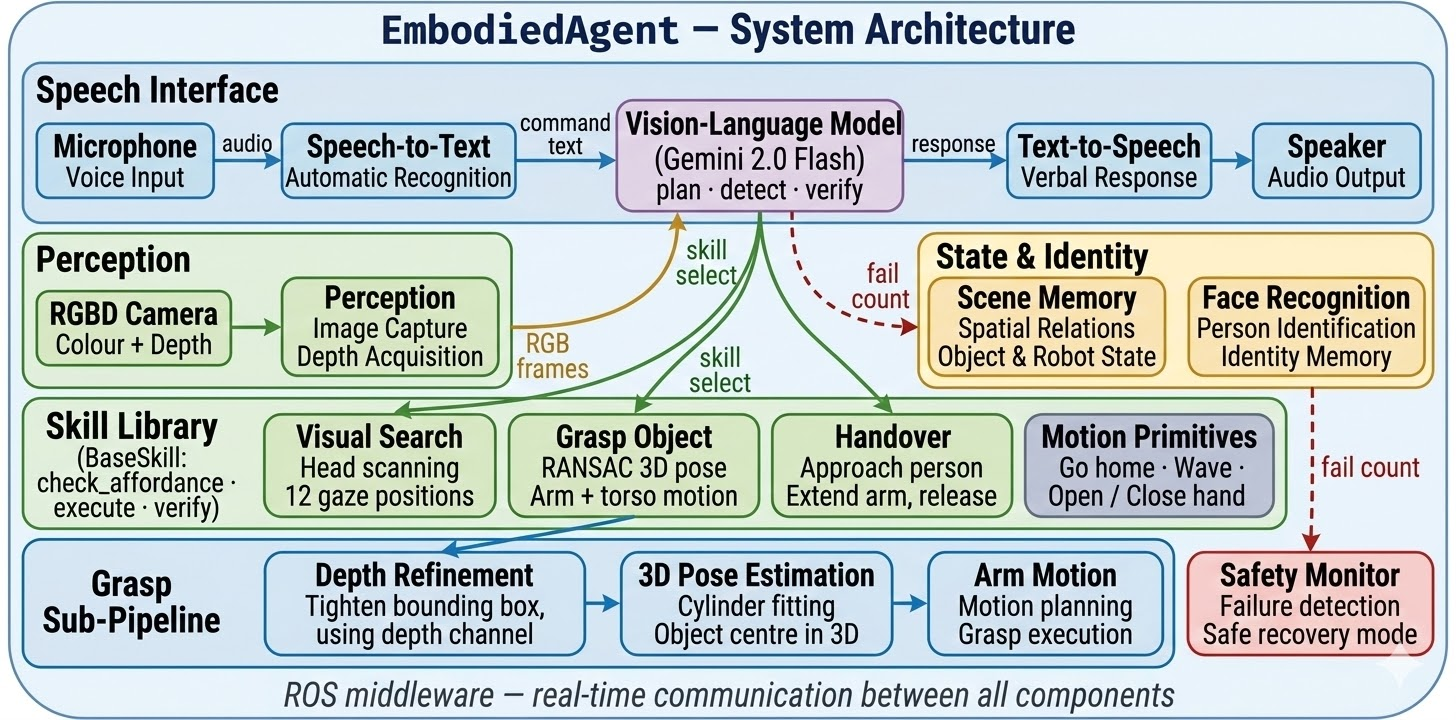
\includegraphics[width=\textwidth,height=0.32\textheight,keepaspectratio]{unnamed.jpg}
\caption{\textbf{System architecture.} The \textsc{EmbodiedAgent} orchestrates a
continuous perception-reasoning-action loop: STT parses voice commands,
the \VLM{} (Gemini~2.0~Flash) simultaneously detects objects and selects skills,
the \SM{} injects live spatial context and updates its scene ontology,
and the skill library executes on the TIAGo hardware via ROS.
The \FM{} microservice runs on the host machine and communicates over HTTP~(port~5002).}
\label{fig:arch}
\end{figure*}

The \textsc{EmbodiedAgent} (Fig.~\ref{fig:arch}) implements a neuro-symbolic
VLA architecture structured around three layers:
\textit{(i)}~a \textbf{neural perception-reasoning layer} (\VLM, Gemini 2.0 Flash)
that processes RGB images and language to select actions;
\textit{(ii)}~a \textbf{symbolic ontology layer} (\SM) that maintains the
agent's semantic world model and injects it into every VLM inference;
and \textit{(iii)}~a \textbf{physical action layer} (skill library, ROS/MoveIt)
that grounds language decisions in physical robot motions.
On each agent cycle, a voice command is transcribed, the \VLM{} queries the
scene with the current ontological context from \SM{}, object memory and
spatial relations are updated, and the selected skill is dispatched.
A safety subsystem monitors consecutive failures and triggers a safe-mode
sequence after three errors, preventing hardware damage.

%--------------------------------------------------------------------
\subsection{Speech Interface}
\label{sec:speech}

Voice commands are transcribed using a dual-engine pipeline: a local
Whisper model serves as the primary recogniser, with a cloud speech API
as fallback when the local model is uncertain.
The robot responds through the PAL TTS system, giving spoken feedback
after each action.

%--------------------------------------------------------------------
\subsection{VLM Reasoner (\VLM)}
\label{sec:vlm}

\VLM{} wraps Gemini~2.0~Flash and serves as the agent's cognitive core.
Given a voice command $u$, the current camera image $\mathbf{I}$, and the
semantic context $\text{ctx}$ from \SM{}, a single API call returns:
\begin{equation}
  \mathcal{V}(u,\,\mathbf{I},\,\text{ctx})
  \;\longrightarrow\;
  \bigl\{\,\texttt{skill},\;\texttt{params},\;\texttt{rationale},\;
            D\,\bigr\}
  \label{eq:vlm}
\end{equation}
where $D$ is the set of detected objects with bounding boxes and labels.
The model thus acts simultaneously as an open-vocabulary detector and a
task planner — no separate perception module is required.
The rationale $\rho$ returned alongside the skill choice is preserved and
used to seed the more specific object-grounding prompt at grasp time
(Section~\ref{sec:grasp}), propagating the agent's intent downward through
the execution stack.

%--------------------------------------------------------------------
\subsection{Semantic World Model (\SM)}
\label{sec:state}

\SM{} is the agent's \textit{semantic world model}
— the symbolic layer of the neuro-symbolic architecture.
It accumulates evidence from every VLM inference step and from the robot's
own sensors (joint state and odometry), maintaining a live picture of
what has been seen, where, and in what relation to other objects.
This replaces the static, offline-built RDF graph of~\cite{eladdachi2025llm}
with a belief state that evolves as the scene changes.

\subsubsection{Object memory.}
For every detected object class $c$, the \SM{} maintains a structured
memory entry $\mathcal{M}[c]$ recording: the last detected bounding box,
the robot's odometric pose at the time of last sighting, the number of
times the object has appeared in the session, the current confidence score,
the set of active spatial relations, and a named location label.
Entries older than five minutes are excluded from the VLM context,
preventing the agent from acting on stale observations.

\subsubsection{Automatic spatial relation inference.}
Spatial relations are inferred from 3D object positions in the robot's
\texttt{base\_footprint} frame, obtained by back-projecting depth pixels
through camera intrinsics and a TF transform.
These geometric base facts seed a \textbf{forward-chaining rule engine}
that derives higher-order symbolic facts to fixpoint:
\begin{compactitem}
  \item \emph{Geometric:} \texttt{left\_of}, \texttt{above}, \texttt{near\_3d},
        \texttt{reachable} (arm-workspace check), \texttt{on\_table}.
  \item \emph{Derived:} \texttt{can\_grasp}$\leftarrow$\texttt{reachable}$\wedge$\texttt{graspable};
        \texttt{handover\_possible}$\leftarrow$\texttt{holding}$\wedge$\texttt{near(robot,person)};
        transitivity closure for \texttt{left\_of}, \texttt{in\_front\_of}.
  \item \emph{VLM semantic:} the model's \texttt{semantic\_facts} output
        (e.g., \texttt{bottle\_is\_open}, \texttt{person\_is\_reaching})
        is merged into the fact base each cycle, completing the neuro-symbolic loop.
\end{compactitem}
Self-referential pairs are filtered to prevent degenerate facts.
The full derived fact base $\mathcal{G}$
is serialized as structured text and prepended to each VLM prompt:
\begin{quote}\small\itshape
Gripper: holding:bottle \textbar{} Location: table\_area \textbar{}
Relations: bottle left\_of cup, cup near box \textbar{}
Memory: cup (3$\times$, 12\,s ago) \textbar{}
History: search\_with\_head\,\checkmark
\end{quote}

%--------------------------------------------------------------------
\subsection{Face Recognition (\FM)}
\label{sec:face}

\FM{} runs as a separate microservice, decoupling face inference from the
main ROS process.
It encodes detected faces as compact embedding vectors and matches them
against a session memory using Euclidean distance: a face is recognised
if its distance to a stored embedding falls below a fixed threshold.
When a known person is seen, the robot greets them by name.
When an unfamiliar face appears, the agent initiates a brief introduction
dialogue — it asks for the person's name, listens via STT, uses the VLM
to parse the response, and stores the face for the rest of the session.

%--------------------------------------------------------------------
\subsection{Active Visual Search (\texttt{search\_with\_head})}
\label{sec:search}

\begin{figure}[t]
\centering
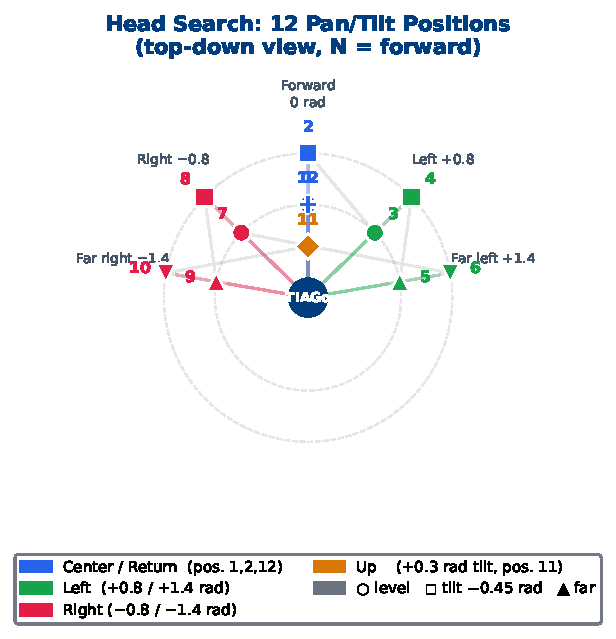
\includegraphics[width=\columnwidth]{figs/fig3_headscan.pdf}
\caption{\textbf{Head scan pattern.}
The robot visits twelve pan/tilt head positions sequentially, running
a VLM detection query at each stop; search ends as soon as the target
is found.}
\label{fig:search}
\end{figure}

When the target is not visible in the initial view,
the active search skill (Fig.~\ref{fig:search}) systematically pans
and tilts TIAGo's head through twelve positions covering the full
workspace.
After settling at each position, the VLM is queried for the target
object; if found, the search ends and the detection is handed off to
the grasping pipeline.
For person targets, an additional check confirms that a face is visible
in the upper portion of the detected bounding box — preventing
false positives on feet or torsos — and adjusts the head tilt if needed.

%--------------------------------------------------------------------
\subsection{Object Grasping Pipeline}
\label{sec:grasp}

\begin{figure*}[t]
\centering
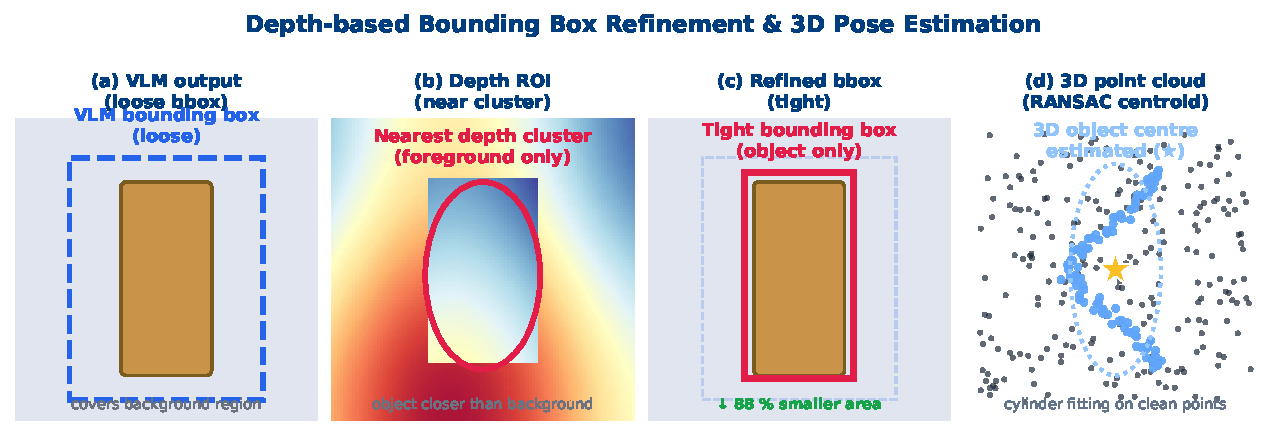
\includegraphics[width=\textwidth]{figs/fig4_depth.pdf}
\caption{\textbf{Depth-based bounding box refinement.}
The VLM produces a semantically correct but spatially loose bounding box (a).
Depth pixels within that region are filtered to the nearest foreground cluster (b),
yielding a tight box that encloses only the object (c).
The resulting clean point cloud is fed to RANSAC cylinder fitting (d).}
\label{fig:refine}
\end{figure*}

The grasping pipeline (Fig.~\ref{fig:refine}) takes the agent from
language-level object reference to physical contact in four stages.

\subsubsection{Context-grounded detection.}
Before querying the VLM for a precise bounding box, the skill assembles
a disambiguation prompt that combines the agent's original rationale $\rho$
with the spatial relations currently held in \SM{}:
\begin{quote}\small\itshape
``\{class\}. The operator selected: [\textit{rationale}] | Spatial: [\textit{relations}].
Return ONLY that one object.''
\end{quote}
This grounds the detection in the agent's broader reasoning context,
helping distinguish between multiple instances of the same class.
The resulting bounding box is cached and reused across all depth frames
to ensure a consistent object selection throughout pose estimation.

\subsubsection{Depth-based bounding box refinement.}
VLM bounding boxes are semantically accurate but spatially coarse —
they often include table surface and background pixels.
To address this, we isolate the nearest foreground depth cluster within
the VLM box: depth pixels within a tolerance of 12\,cm above the nearest
point in the region are retained, and the refined bounding box is their
axis-aligned enclosure.
This produces a tight crop around the object without any segmentation model.

\subsubsection{3D pose estimation.}
Pixels within the refined box are back-projected to 3D using camera
intrinsics and a coordinate transform to the robot base frame.
RANSAC fits a vertical cylinder to the resulting point cloud, which works
well for bottles and cans; flat or box-shaped objects fall back to a
median centroid estimate.
Five successive estimates are averaged for stability, and a reachability
check discards poses that fall outside the robot's arm workspace.

\subsubsection{Arm execution.}
MoveIt plans a collision-free trajectory to a pre-grasp pose 20\,cm
above the object.
Final descent is performed by lowering the torso lift joint in a straight
vertical line, which guarantees a top-down approach without IK divergence
near the table surface.
After grasping, the trunk rises to clear the workspace before the robot
returns to its home pose.

%--------------------------------------------------------------------
\subsection{Object Handover}
\label{sec:handover}

The handover skill detects the person in the current camera frame,
back-projects their bounding box centroid to 3D, and commands MoveIt to
extend the arm toward the person at a fixed handover height of 0.85\,m,
capped at 0.62\,m in depth to stay within the reachable workspace.
Stale collision objects from the prior grasp are cleared before planning.
The robot announces the handover via TTS, waits 4\,s for the person to
take the object, then opens the gripper and returns home.


%============================================================================
\section{Discussion}
\label{sec:discussion}

\paragraph{Neuro-symbolic agent loop.}
The key architectural insight is the separation of \textit{neural} perception
(VLM) from \textit{symbolic} reasoning (\SM): the VLM produces rich,
open-vocabulary observations, while the \SM{} maintains a structured,
interpretable world model that constrains and grounds the next VLM call.
This closed loop turns a stateless VLM API into a stateful, session-aware
agent — capable of tracking what the robot is holding, what objects it has
seen, and how they relate, across an entire interaction.

\paragraph{Live semantic ontology vs.\ static knowledge graphs.}
Unlike the static RDF graph of~\cite{eladdachi2025llm} — which requires
offline construction and cannot reflect scene changes — the \SM{} updates
its scene ontology at every inference step from live visual evidence.
This is critical in interactive manipulation: once an object is grasped,
the \SM{} immediately registers the change in gripper state and
propagates it into the next prompt, preventing the agent from attempting
to re-grasp an already-held object.
The 5-minute recency window is configurable; a shorter timeout is preferable
in highly dynamic environments.

\paragraph{VLM as unified cognitive module.}
Querying a single model for both visual grounding and skill selection
eliminates the latency and error cascade of a detect-then-plan pipeline.
The rationale returned alongside each skill choice acts as structured
chain-of-thought that seeds the subsequent grasp-level disambiguation
prompt, propagating the agent's high-level intent down to the physical
execution layer — a lightweight form of hierarchical planning.

\paragraph{Grounding language in physical space.}
VLM bounding boxes are semantically accurate but spatially loose.
The depth-based refinement step bridges the gap between language-level
perception and physical-level manipulation: by isolating the nearest
foreground cluster, it produces a tight bounding volume that grounds the
agent's object reference in metric 3D space, without any segmentation model.

\paragraph{Computational footprint and API dependency.}
The entire inference pipeline runs without a local GPU, with all ROS
control, RANSAC, and MoveIt planning executed on a standard laptop CPU.
This lowers the hardware barrier for deployment on commodity service robots.
The trade-off is a dependency on cloud API availability: Gemini 2.0 Flash
round-trip latency is the primary bottleneck, and network outages represent
a single point of failure.
Deploying a quantised local VLM would eliminate this dependency at the cost
of higher latency — a reasonable path for safety-critical or offline deployments.

%============================================================================
\section{Limitations and Future Work}
\label{sec:limitations}

The current system has several identifiable limitations.
\textbf{Geometry model.}
Cylindrical RANSAC fails on flat, irregular, or handle-bearing objects;
future work could add a superquadric fitting fallback or learn
object-class-specific grasp templates from a small offline dataset.
\textbf{Static named locations.}
Navigation targets are hardcoded; replacing them with a semantic 3D map
(e.g., SayPlan-style~\cite{rana2023sayplan}) would support multi-room
deployment without manual calibration.
\textbf{API dependency.}
Cloud VLM availability is a single point of failure.
Deploying a quantised local model (LLaVA-7B or similar) would provide
offline resilience, at the cost of higher latency and a GPU requirement.
\textbf{Cluttered scenes.}
The nearest-depth cluster assumption breaks when multiple objects occupy
the same depth band, potentially merging two adjacent objects into a single
refined bbox. Integrating instance segmentation — for example, the incremental
learning module of Kenai~et~al.~\cite{kenai2025neuro} — would resolve
per-object boundaries in such cases.
\textbf{Memory recency.}
The 5-minute recency window for object memory is appropriate for a static
tabletop, but too long for highly dynamic scenes where objects are frequently
moved by a user. A shorter, task-adaptive timeout would better reflect actual
scene state in interactive environments.
\textbf{Evaluation scope.}
The system has been demonstrated in a controlled laboratory environment with
stable lighting; further testing in unstructured, changing environments
(e.g., care homes, offices) is needed to assess real-world robustness.

%============================================================================
\section{Conclusion}
\label{sec:conclusion}

We presented a neuro-symbolic embodied agent for the TIAGo mobile
manipulator that closes the full loop from free-form voice commands to
physical object handover, without a local GPU and without retraining
for new object categories.
The integration demonstrates three practical design choices:
\textit{(i)}~a live semantic state manager (\SM{}) that injects structured
perceptual context into every VLM prompt, enabling session-persistent
multi-instance disambiguation without weight updates;
\textit{(ii)}~a single VLM call for both open-vocabulary detection and
skill selection, replacing the separate detector\,+\,planner architecture
of prior work;
and \textit{(iii)}~a depth-based foreground extraction step that improves
3D localisation from loose VLM bounding boxes without segmentation masks.

The work builds on the LISSI line of neuro-symbolic
systems~\cite{abdelkawy2021ral,eladdachi2025llm}, extending it from
static knowledge-assisted control to a fully deployed agent capable of
physical manipulation and object handover on a real mobile platform.
We hope this integration serves as a practical blueprint for deploying
cloud-based VLMs in embodied robotics settings that do not have access
to local GPU hardware.

%============================================================================
\bibliographystyle{unsrtnat}
\bibliography{references}

\end{document}
